\newpage
\section*{Earls of Ravnica}

\subsection*{The \texttt{district} module}

I have chosen to use the \texttt{gen\_statem} behaviour for my implementation. An individual district is its own state machine, and so, it makes sense to model it as such using the \texttt{gen\_statem} behaviour in Erlang. The callback mode i have used is \texttt{state\_functions}. That is, for each state of the district I define a callback function to handle the variaous events. This is, in my opinion, more convenient than using \texttt{handle\_event\_function}, since you can have a dedicated function per state.

I will try to cover only the most essential parts of my implementation, leaving the rest as something to read in the source.

\paragraph{Creating a district} In order to create a district, and thus initialize a new state machine, I have implemented \texttt{create} by simply calling \texttt{gen\_statem:start}, giving the module name, description, and the empty list as arguments. The \texttt{init} callback function sets the inital state to \texttt{under\_configuration} and passes the initial state data. Since we are working with neighbours, creatures, a trigger, and a description as the state data, the data is represented by a four-tuple consisting of a \texttt{map(atom() => passage())}  for the neighbours, a \texttt{map(creature\_ref() => creature\_stats())} for the creatures, simply a \texttt{trigger()} function for the trigger, and a string for the description.

% \paragraph{Getting the description} This simply sends a call to the given district, which will then return the description from the state data no matter the state in which it is.

\paragraph{Connecting districts} \texttt{connect} sends a call to the given district, passing on the action and the destination. Representing the connections to the neighbours as a map, it is easy see if the action is already taken; simply ask if the action already exists as a key, and if it does, return the appropriate error. Else, put it into the map with the destination as the value and return \texttt{ok}.

\paragraph{Activating a district} This has been a bit tricky, and I have tried a few solutions before choosing to do it this way. When a district, which is under configuration, is activated, it immediately goes to the \texttt{under\_activation} state and forces the next event to be an internal event where the district then activates all of its neighbours. When each activation of the neighbours has returned a value, the district checks if any activation has been impossible. If this is the case, the district itself can't be activated. In order to avoid blocking the processes, each path that is activated keeps track of a list of visited districts. Thus, everytime a district is activating its neighbours, it chooses to ignore the ones that have already been visited. This also takes care of cycles, however, even without the list of visited districts, cycles are handled automatically; \texttt{activate} terminates the chain of calls when it is already under activation.

If there is a path from the root district being activated to some district that can't be activated, the root district also fails. Thus, I assume that it is possible to activate a part of a territory that does not include the root being activated. On Figure \ref{fig:activate} I have tried to illustrate my assumption about how \texttt{activate} would work. A, B, and (trivially) C fail to activate since they all have a path to a district that can't be activated. However, D and E are successfully activated.
\begin{figure}
  \centering
  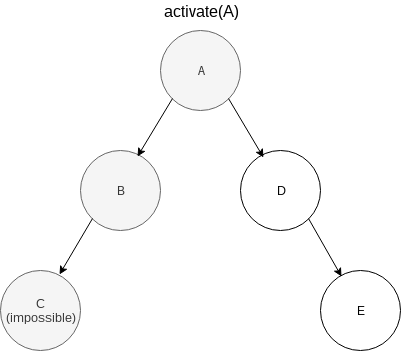
\includegraphics[width=0.5\textwidth]{figures/activate}
  \caption{Activating a district A with one path to a district that can't be activated and one path without problems.}\label{fig:activate}
\end{figure}

\paragraph{Entering a district} This sends a call to the district, passing the creature wanting to enter. The district simply checks to see if the reference is already a key in the creature map, and if not, applies the \texttt{entering}-trigger to the creature entering and the creatures already in the district. The result then represents the  new map of creatures in the state data.

The way the well-formedness of the trigger is checked is as follows. A new process applying the trigger is spawned, which sends a message back with the result. This allows me to use the \texttt{after}-timeout when receiving the result. If there is no result within 2 seconds, the input to the trigger is simply returned. The spawned process calls the trigger and catches any exception that may occur --- if this happens, the input is returned. If there is a response within 2 seconds, the check proceeds by ensuring that the result is a tuple, and that all the creature references are the same. If all is well, the new data is returned.

\paragraph{Taking action} This sends a call to the district, passing the creature reference and the action. The district makes sure that the creature is actually in the map of contained creatures and that the action exists in the map over neighbours. If so, the \texttt{leaving}-trigger is applied to the creature leaving and the creatures staying in the district, and \texttt{enter} is called on the destination. If all goes well, the creature is moved. One special case is when the action is an edge to the same district; this would, again, block everything. Thus, if the destination is the same as the current district, the \texttt{entering}-trigger is applied locally and the state data is updated accordingly.

This solution may not be the most elegant since it repeats some code from \texttt{enter}. However, given the problems that arise when handling self loops, this solution is a very simple way to avoid blocking the process.

\paragraph{Shutting down a district} This works much in the same way as \texttt{activate}. After sending the required message to the \texttt{NextPlane} argument, the district immediately goes to the \texttt{shutting\_down} state and forces an internal event that makes it shut down its neighbours. After they have all been visited, I use the \texttt{gen\_statem:stop}.


\subsection*{QuickCheck \texttt{district}}
